\section{Results}
Table \ref{tab:ChatbotAnswers} depicts how the chatbot answered each question for each vector store. Refer to 
Table \ref{tab:GoldenDataset} for the corresponding question to each ID.

\begin{longtable}{ | p{0.05\linewidth} | p{0.2\linewidth} | p{0.2\linewidth} | p{0.2\linewidth} | p{0.2\linewidth} | }
    \hline
    \cellcolor{blue!25} ID & \cellcolor{blue!25} FAISS & \cellcolor{blue!25} SmallChunks & \cellcolor{blue!25} BigChunks & \cellcolor{blue!25}HugeChunks \\
    \hline
    \cellcolor{blue!25} 1 & \cellcolor{red!25} Wrong & \cellcolor{red!25} Wrong  
                          & \cellcolor{red!25} Wrong & \cellcolor{green!25} Correct\\
    \hline
    \cellcolor{blue!25} 2 & \cellcolor{red!25} Wrong & \cellcolor{red!25} Wrong
                          & \cellcolor{red!25} Wrong & \cellcolor{red!25} Wrong\\
    \hline 
    \cellcolor{blue!25} 3 & \cellcolor{green!25} Correct & \cellcolor{red!25} Wrong
                          & \cellcolor{green!25} Correct & \cellcolor{green!25} Correct\\
    \hline 
    \cellcolor{blue!25} 4 & \cellcolor{green!25} Correct & \cellcolor{yellow!25} Questionable 
                          & \cellcolor{green!25} Correct & \cellcolor{green!25} Correct \\
    \hline 
    \cellcolor{blue!25} 5 & \cellcolor{red!25} Wrong & \cellcolor{red!25} Wrong 
                          & \cellcolor{red!25} Wrong & \cellcolor{green!25} Correct\\
    \hline 
    \cellcolor{blue!25} 6 & \cellcolor{green!25} Correct & \cellcolor{green!25} Correct 
                          & \cellcolor{red!40} "I don't know" & \cellcolor{green!25} Correct\\
    \hline 
    \cellcolor{blue!25} 7 & \cellcolor{yellow!25} Questionable & \cellcolor{red!25} Wrong 
                          & \cellcolor{red!25} Wrong & \cellcolor{green!25} Correct \\
    \hline 
    \cellcolor{blue!25} 8 & \cellcolor{red!25} Wrong & \cellcolor{red!25} Wrong
                          & \cellcolor{green!25} Correct & \cellcolor{red!25} Wrong \\
    \hline
    \cellcolor{blue!25} 9 & \cellcolor{red!25} Wrong & \cellcolor{red!25} Wrong
                          & \cellcolor{red!25} Wrong & \cellcolor{green!25} Correct \\
    \hline 
    \cellcolor{blue!25} 10 & \cellcolor{green!25} Correct & \cellcolor{green!25} Correct 
                           & \cellcolor{green!25} Correct & \cellcolor{green!25} Correct\\ 
    \hline
    \cellcolor{blue!25} & \cellcolor{yellow!25} \textbf{40\%} & \cellcolor{red!25} \textbf{20\%} 
    & \cellcolor{yellow!25} \textbf{40\%} & \cellcolor{green!40} \textbf{80\%} \\
    \hline
    \caption{The performance of the chatbot with each vector store.}\label{tab:ChatbotAnswers}
\end{longtable}

\para G-Eval assigns a score to each of the chatbot's answers to the golden dataset questions, where scores under 0.5 are deemed to be 
incorrect. However, answers marked as 'Questionable' were answers that were technically correct after manual inspection despite 
G-Eval labelling them as incorrect. This showcases in part the occasional unreliability of LLMs even in judging contexts 
such as G-Eval. 

\para The questionable judgments were with Questions 3 and 4 on the smallest chunk-size vector store, depicted in Figures \ref{fig:Questionable1}
and \ref{fig:Questionable2}.

\begin{figure}[H]
    \centering
    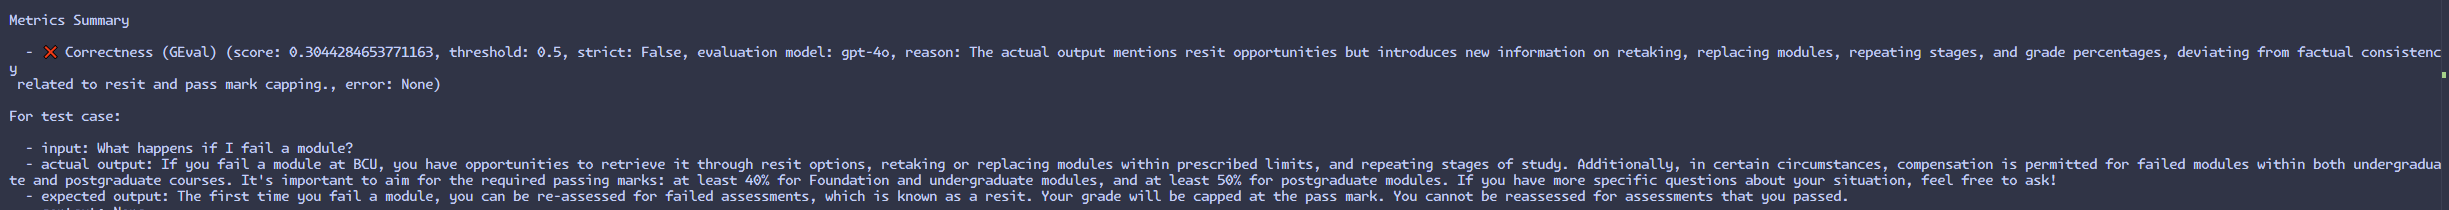
\includegraphics[width=\textwidth]{Evaluation/FAISS-SmallChunks/Questionable1.png}
    \caption{The G-Eval judgment of the chatbot's response to Question 3 using the FAISS-SmallChunks vector store. \label{fig:Questionable1}}
\end{figure}

\noindent The answer provided here was very narrowly under G-Eval's 0.5 judgment threshold meaning that it was deemed to be incorrect, 
with the gpt-4o evaluator LLM stating that unsupported information was introduced. However, upon manual inspection, the information 
provided by the chatbot in response to this question is correct. 

\para There is a similar occurrence in the response to Question 4 using this vector store, as depicted in Figure \ref{fig:Questionable2}.

\begin{figure}[H]
    \centering
    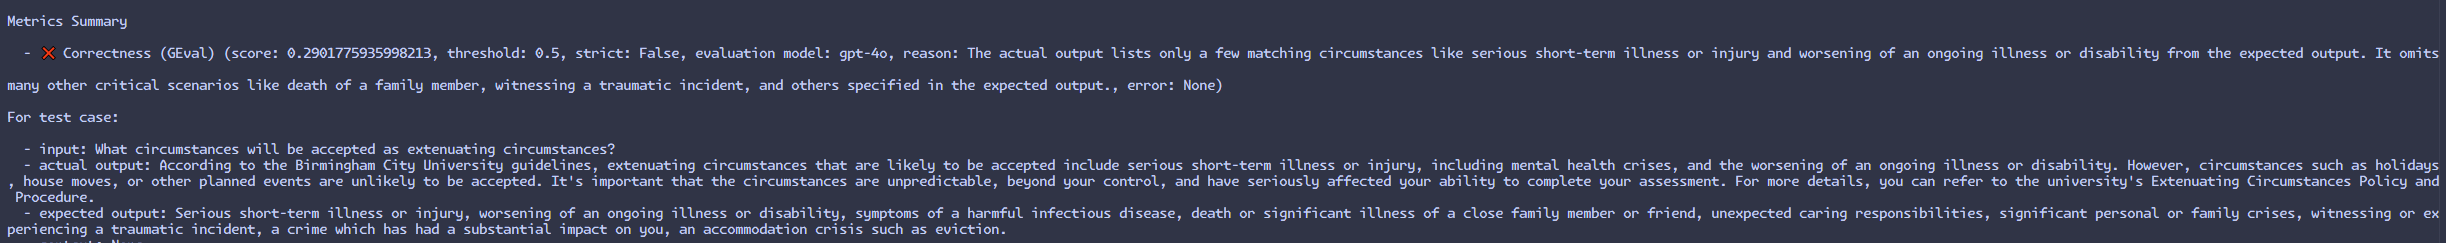
\includegraphics[width=\textwidth]{Evaluation/FAISS-SmallChunks/Questionable2.png}
    \caption{The G-Eval judgment of the chatbot's response to Question 4 using the FAISS-SmallChunks vector store. \label{fig:Questionable2}}
\end{figure}

\noindent G-Eval uses the expected answer verbatim, meaning that with the long list of options provided in the expected answer to Question 4, 
G-Eval expected the chatbot to respond with every option as stated in its response: "It omits many other critical scenarios ... specified in the expected output". While this is expected behaviour of G-Eval, it proves that manual evaluation can still 
be more suitable in specific scenarios, as the answer given by the chatbot here was manually deemed to be of good quality despite not listing 
every possible scenario.

\para There were also two more noteworthy observations, both with the FAISS-BigChunks vector store, with its response to Question 6 being 
"I don't know", and the response to Question 8 being the only correct response of all four vector stores, even including the best-performing
vector store.

\begin{figure}[H]
    \centering
    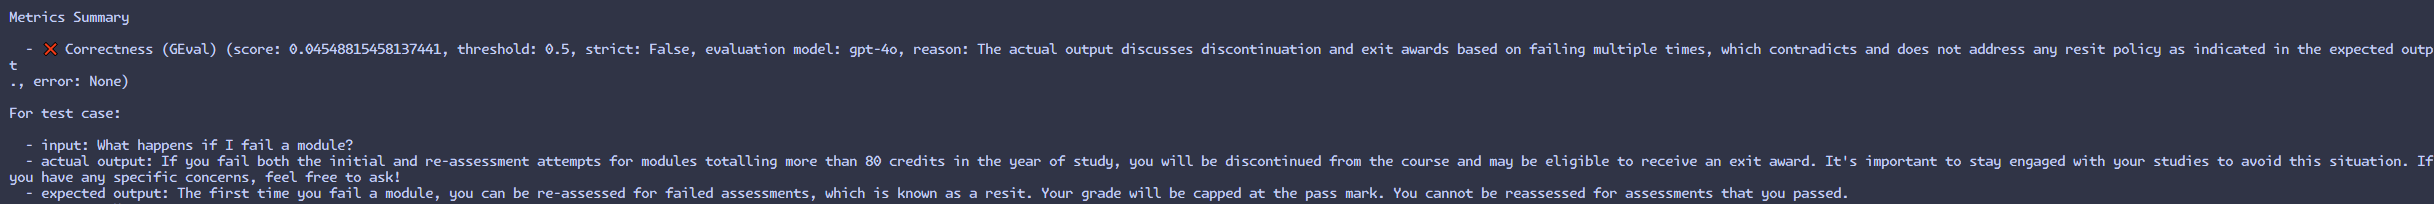
\includegraphics[width=\textwidth]{Evaluation/FAISS-BigChunks/Incorrect4.png}
    \caption{The G-Eval judgment of the chatbot's poor response to Question 6 using the FAISS-BigChunks vector store. \label{fig:ChatbotIDK}}
\end{figure}

\noindent The chatbot's total failure to answer the question using this vector store signifies a potential issue in the retrieval tool, yet every 
other vector store could successfully retrieve the passing grades in question. It is possible that while the PDFs were being split into chunks 
for this vector store specifically, the information required for this question was split over multiple chunks despite the large size and overlap,
meaning the similarity search could not find a suitable answer. The chatbot's system prompt states that it must respond with "I don't know" if it 
is unable to retrieve relevant context, and this is displayed clearly within this failure.

\begin{figure}[H]
    \centering
    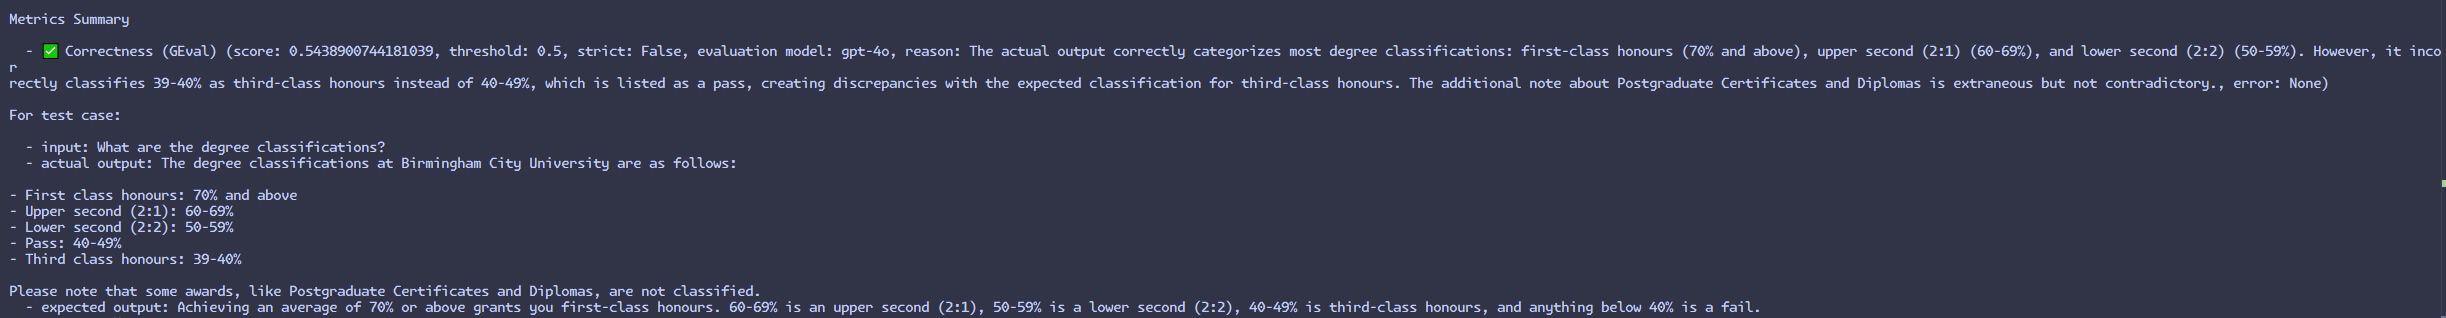
\includegraphics[width=\textwidth]{Evaluation/FAISS-BigChunks/UniqueCorrect.png}
    \caption{The G-Eval judgment of the uniquely good response to Question 8. \label{fig:UniqueCorrect}}
\end{figure}

\noindent Intriguingly, this particular vector store was the only one where the information needed to answer the question about degree classifications 
was successfully retrieved for a response. It is possible that the question itself may have been misinterpreted when performing semantic similarity searches on the other vector stores, leading them to instead fail on this question as shown in Figure \ref{fig:WrongAnswer2}.

\subsection{Best-performing system}
\para Images of the G-Eval outputs for each incorrect answer for all vector stores can be found in \href{https://github.com/LewGoesB00M/CMP6200/tree/main/LaTeX/.images/Evaluation}{the project's Github repository}, though this section will focus on the best-performing vector store, which was 
FAISS-HugeChunks.

\begin{figure}[H]
    \centering
    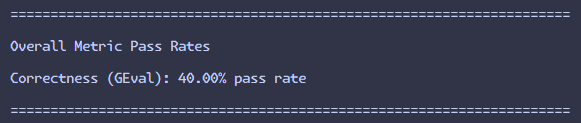
\includegraphics[width=\textwidth]{Evaluation/FAISS-HugeChunks/Overall.png}
    \caption{Overall G-Eval results against the "FAISS-HugeChunks" vector store. \label{fig:EvalResults}}
\end{figure}

\noindent On the ten test cases on various academic policies and information used in evaluating the chatbot,
80\% were answered correctly according to G-Eval. Figures \ref{fig:WrongAnswer1} and \ref{fig:WrongAnswer2} depict 
the two queries where the chatbot failed to give a suitable answer.

\begin{figure}[H]
    \centering
    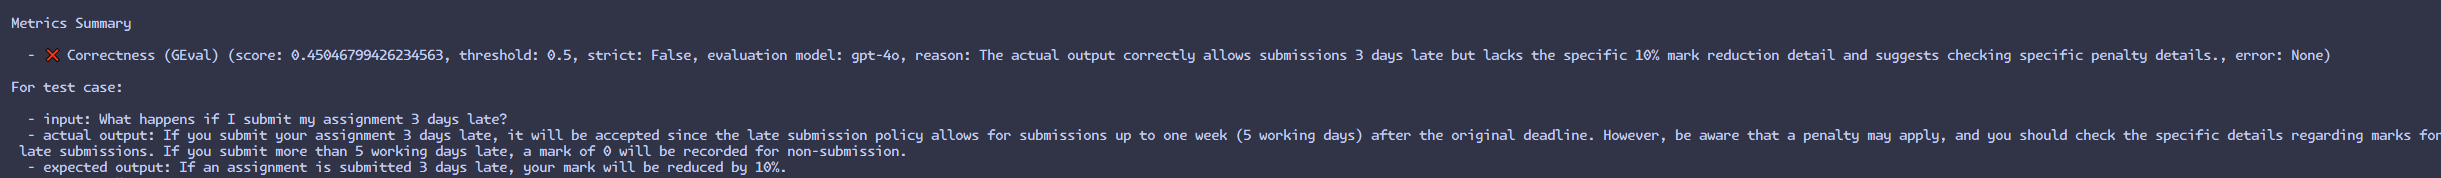
\includegraphics[width=\textwidth]{Evaluation/FAISS-HugeChunks/Incorrect1.png}
    \caption{The first incorrect answer, with the chatbot answering incorrectly. \label{fig:WrongAnswer1}}
\end{figure}

\noindent This question was answered incorrectly due to the chatbot's misinterpretation of the related policy. Work submitted \textbf{up to} 
1 hour after a deadline does \textbf{not} receive any grade penalty, though the chatbot likely read that work submitted \textbf{between 1 hour and 
24 hours} after a deadline \textbf{does} incur a penalty. As such, this misinterpretation lead to the question being answered incorrectly.

\begin{figure}[H]
    \centering
    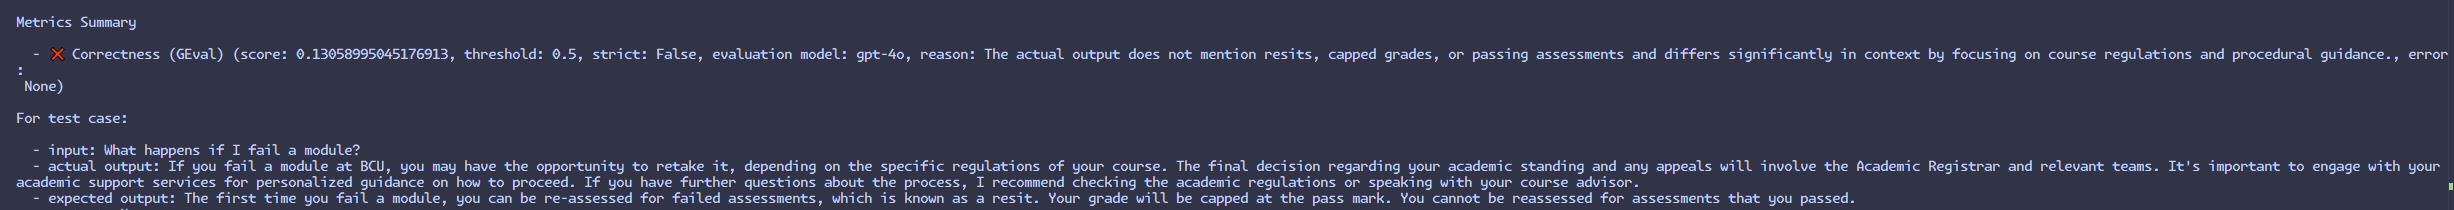
\includegraphics[width=\textwidth]{Evaluation/FAISS-HugeChunks/Incorrect2.png}
    \caption{The second incorrect answer, with incorrect information retrieval. \label{fig:WrongAnswer2}}
\end{figure}

\noindent The chatbot retrieving information that isn't directly relevant for this question implies an error in the retrieval tool. 
This could likely be due to the format of each policy document, with the information requested here (degree thresholds) being stored in
a table, depicted in Figure \ref{fig:WrongAnswer2Snippet}.

\begin{figure}[H]
    \centering
    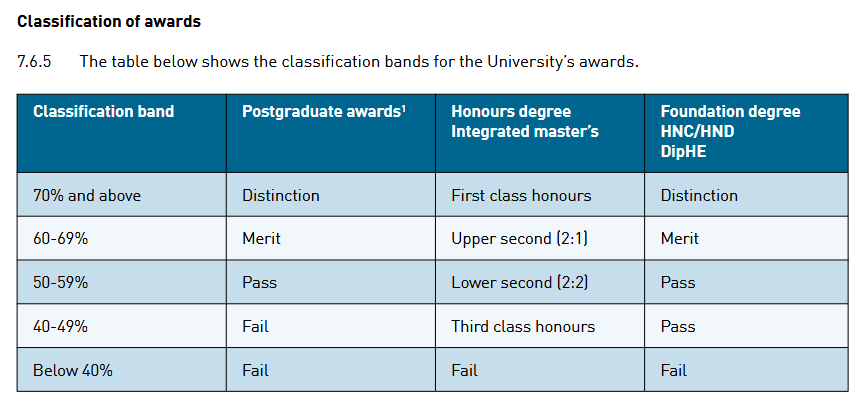
\includegraphics[width=\textwidth]{Evaluation/WrongAnswerPolicy.png}
    \caption{The snippet of the Academic Regulations that should have been referenced. \autocite{bcuPoliciesProcedures} \label{fig:WrongAnswer2Snippet}}
\end{figure}

\noindent The 'PyPDFLoader' class in LangChain, which was used when storing all University data, can sometimes misinterpret tables. 
This may in turn have created issues with the semantic search performed on the FAISS DB, leading to this question going unanswered as 
the search was unable to identify each degree classification.